\section{失败模式：什么信息最容易在视觉压缩里丢失}

本章的结论很直接：MemOCR 的强项来自版面显著性分配，它的主要风险也来自同一处。一旦模型把真正决定答案的细粒度关系放进低显著区域，或者在有限画布里写入过多内容，压缩后的视觉记忆就会从“可读的摘要”退化成“看似完整、实际难读”的信息堆。

\begin{importantbox}{失败模式的总括}
视觉记忆的容量边界可以写成一个简单约束：画布面积、字体大小、下采样倍率、image token 数共同决定可读性。MemOCR 能调节信息密度，代价是它必须学会判断哪些信息值得占据高显著位置。判断错了，错误会沿着 memory drafting、rendering、memory reading 一路传到 final answer。
\end{importantbox}

\subsection{Failure Mode A：比较关系被低估}

第一类 failure mode 是比较推理中的 fine-grained details 丢失。讲者给出的例子是比较两个人谁更 professional。这个问题表面上只是在问 A 与 B 的高低，真正的证据却常常藏在相对关系里：两人的角色、经历、作品、评价标准，以及这些事实如何共同支持“更 professional”的判断。

MemOCR 在压缩时可能会把两个人名或头衔放到较高的 heading level。heading level 在视觉上很醒目，类似一张白板上字号最大的标题。问题在于，人名和标题本身信息增益有限；决定答案的证据是“谁在什么维度上更强、为什么更强”。如果这些相对关系被放到辅助信息区域，也就是 detail area 或其他较低显著区域，高压缩后模型读到醒目的外壳，却读漏了判断所需的内核。

\begin{warningbox}{比较题的隐蔽风险}
比较题比事实抽取更容易失效，因为答案依赖关系结构。单个事实像一张身份证号码，放错位置仍可能被检索；比较关系像天平两端的砝码，缺少任意一端或缺少比较准则，最终判断就会偏移。
\end{warningbox}

从第一性原理看，这个问题是“价值估计错误”。模型需要为每条信息估计它对答案的边际贡献。可以用讲义抽象表达为：

$$
u(I_i, Q) = \Delta \operatorname{Score}(Q \mid I_i)
$$

其中：

\begin{itemize}
  \item $I_i$ 表示第 $i$ 条候选记忆信息；
  \item $Q$ 表示当前或潜在问题；
  \item $u(I_i, Q)$ 表示这条信息对回答问题 $Q$ 的效用；
  \item $\Delta \operatorname{Score}$ 表示加入该信息后答案质量的增量。
\end{itemize}

比较推理的困难在于，单看某条信息时它可能很普通，和另一条信息组合后才变得关键。例如“甲有高级职位”与“乙完成了更专业的实际项目”分别看都像普通事实，放到“谁更 professional”这个问题里，它们之间的相对解释才是答案的支柱。

\subsection{Failure Mode B：视觉记忆过载}

第二类 failure mode 是 memory capacity overflow。它发生在模型把过多信息写进同一张视觉记忆图，导致压缩后部分文字可读性急剧下降。讲者举的日期问题很典型：正确答案是 \texttt{2015-02-14}，但模型回答成错误日期。相关信息有时已经写入，问题出在记忆中重复强调了太多内容，整体信息量超过画布和下采样后的可承载范围，最终关键日期在视觉读取阶段变得难以辨认。

\begin{figure}[htbp]
  \centering
  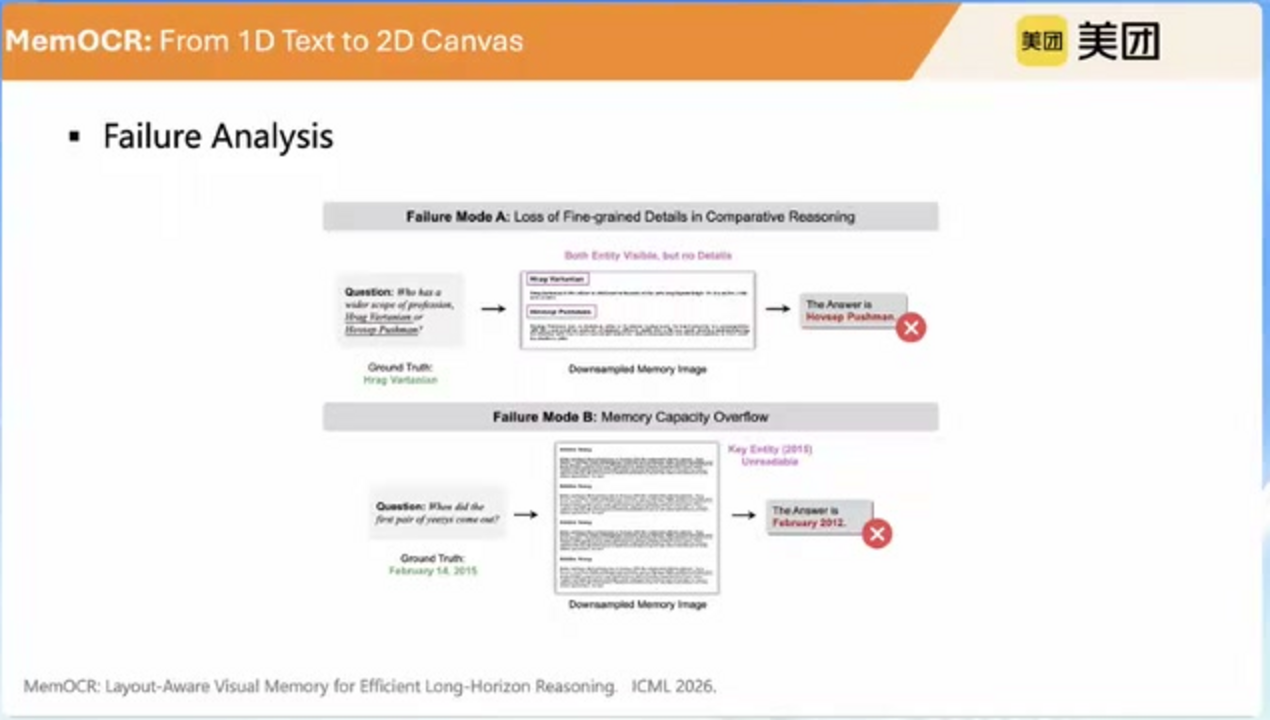
\includegraphics[width=0.86\linewidth,height=0.42\textheight,keepaspectratio]{figures/selected/fig09_failure_analysis.png}
  \caption{Failure Analysis 展示了两类边界：上半部分是比较推理中 fine-grained details 被放到低效区域，导致 final answer 得不到正向支持；下半部分是 memory capacity overflow，信息过密让正确日期在压缩后失去可读性。\protect\footnotemark}
\end{figure}
\footnotetext{视频时间：00:19:30--00:20:00。}

这个失败模式可以用一个容器类比理解。文本压缩像把文件装进一个固定大小的压缩包，视觉记忆像把便签贴到一块白板上。便签数量少时，标题、分区、字号会帮助读者快速定位；便签数量过多时，每张便签只能越写越小，分区仍在，文字已经读不清。视觉布局没有创造无限容量，它只是提供了更灵活的容量分配方式。

为避免把“写得多”误当成“记得好”，可以把视觉记忆的有效容量写成一个约束：

$$
\sum_{i=1}^{n} c(I_i, s_i, \rho_i) \leq C_{\text{readable}}
$$

其中：

\begin{itemize}
  \item $I_i$ 表示写入画布的第 $i$ 条信息；
  \item $s_i$ 表示它的视觉显著性，例如字号、标题层级、位置；
  \item $\rho_i$ 表示压缩强度或写入密度；
  \item $c(I_i, s_i, \rho_i)$ 表示这条信息消耗的可读容量；
  \item $C_{\text{readable}}$ 表示在给定下采样倍率和 image token budget 下仍可被识别的容量上限。
\end{itemize}

该公式是讲义抽象，用来说明边界条件。它强调一个实际工程判断：视觉记忆需要预算控制，不能把所有事实都塞进画布。尤其在极低 memory budget 下，系统要优先保留会改变答案的证据链。

\subsection{从失败模式反推安全使用边界}

两类失败模式共同说明，MemOCR 的使用边界取决于三个问题。

\begin{enumerate}
  \item 信息是否具有明确层级。若任务能区分 crucial area、detail area 和 supporting facts，版面控制更容易发挥作用。
  \item 答案是否依赖细粒度关系。若任务需要比较、排序、因果归因或跨实体关系，系统需要额外保护关系信息。
  \item 压缩后的画布是否仍可读。若图像经过多轮下采样后文字和结构已经难以识别，后续推理训练很难补回底层视觉识别损失。
\end{enumerate}

\begin{knowledgebox}{工程含义}
MemOCR 的安全使用方式需要同时监控“存什么、放哪里、压多狠、读得出吗”。这四个问题对应信息选择、layout control、memory budget、base vision-language model 的识别能力。
\end{knowledgebox}

这也解释了为什么比较问题需要特别处理。一个更稳妥的视觉记忆策略应把“相对关系”当成一等信息，而非把实体名称当成核心信息。例如在 A/B 比较中，画布上应显式保留比较维度、A 的证据、B 的证据、最终判据，而非只把 A 和 B 的标题做大。

\subsection{本章小结}

MemOCR 的失败模式具有机制性，来自视觉记忆的自然边界。Failure Mode A 暴露的是信息价值估计问题：比较关系、相对证据、细粒度判断依据容易被低估。Failure Mode B 暴露的是可读容量问题：画布承载量超过 $C_{\text{readable}}$ 后，正确证据即使写入也可能读不出来。因此，MemOCR 适合做长程记忆压缩，但需要配合关系保护、容量约束和可读性检查。最后一章将把这些边界放回 Q\&A 语境，说明 MemOCR 更适合哪些多模态长程场景，以及压缩边界如何受底层视觉识别能力约束。
